In this section we include multiple examples on defining and simulating models.

\hyperlink{example1}{Example 1} \+: Forward Sensitivities for model with events and discontinuities.

\hyperlink{example2}{Example 2} \+: Forward Sensitivities for m\+R\+N\+A transfection model with bolus injection.

\hyperlink{example3}{Example 3} \+: Steady State Sensitivities.

\hyperlink{example4}{Example 4} \+: Adjoint Sensitivities for J\+A\+K/\+S\+T\+A\+T model with parametric standard deviation.

\hyperlink{example5}{Example 5} \+: Adjoint Sensitivities for m\+R\+N\+A transfection model with bolus injection.

\hyperlink{example6}{Example 6} \+: Adjoint Sensitivities for simple model with analytic solution. \hypertarget{example1}{}\subsection{Example 1}\label{example1}
\hypertarget{example1_def1}{}\subsubsection{Model Definition}\label{example1_def1}
 
% This LaTeX was auto-generated from MATLAB code.
% To make changes, update the MATLAB code and republish this document.











    
    \begin{DoxyCode}
function [model] = example_model_1_syms()
\end{DoxyCode}
\begin{par}
CVODES OPTIONS
\end{par} \vspace{1em}
\begin{DoxyCode}
% set the default absolute tolerance
model.atol = 1e-8;
% set the default relative tolerance
model.rtol = 1e-8;
% set the default maximum number of integration steps
model.maxsteps = 1e4;
% set the parametrisation of the problem options are 'log', 'log10' and
% 'lin' (default).
model.param = 'log10';
\end{DoxyCode}
\begin{par}
STATES
\end{par} \vspace{1em}
\begin{DoxyCode}
% create state syms
syms x1 x2 x3

% create state vector
x = [
x1 x2 x3
];
\end{DoxyCode}
\begin{par}
PARAMETERS ( for these sensitivities will be computed )
\end{par} \vspace{1em}
\begin{DoxyCode}
% create parameter syms
syms p1 p2 p3 p4

% create parameter vector
p = [p1,p2,p3,p4];
\end{DoxyCode}
\begin{par}
CONSTANTS ( for these no sensitivities will be computed ) this part is optional and can be ommited
\end{par} \vspace{1em}
\begin{DoxyCode}
% create parameter syms
syms k1 k2 k3 k4

% create parameter vector
k = [k1 k2 k3 k4];
\end{DoxyCode}
\begin{par}
SYSTEM EQUATIONS
\end{par} \vspace{1em}
\begin{DoxyCode}
% create symbolic variable for time
syms t

xdot = sym(zeros(size(x)));

% piecewise defined function
xdot(1) = -p1*heaviside(t-p4)*x1;
% inhomogeneous
xdot(2) = +p2*x1*exp(-0.1*t)-p3*x2 ;
xdot(3) = -1.5*x3;
\end{DoxyCode}
\begin{par}
INITIAL CONDITIONS
\end{par} \vspace{1em}
\begin{DoxyCode}
x0 = sym(zeros(size(x)));

x0(1) = k1;
x0(2) = k2;
x0(3) = k3;
\end{DoxyCode}
\begin{par}
OBSERVALES
\end{par} \vspace{1em}
\begin{DoxyCode}
y = sym(zeros(1,1));

y(1) = p4 * (x1+x2+x3);
\end{DoxyCode}
\begin{par}
EVENTS this part is optional and can be ommited
\end{par} \vspace{1em}
\begin{DoxyCode}
syms t

% events fire when there is a zero crossing of the root function
event(1) = amievent(x3-x2,0,t);
event(2) = amievent(x3-x1,0,t);
\end{DoxyCode}
\begin{par}
SYSTEM STRUCT
\end{par} \vspace{1em}
\begin{DoxyCode}
model.sym.x = x;
model.sym.k = k;
model.sym.xdot = xdot;
model.sym.p = p;
model.sym.x0 = x0;
model.sym.y = y;
model.event = event;
\end{DoxyCode}
\begin{DoxyCode}
end
\end{DoxyCode}

         \begin{DoxyCode}ans = 
        atol: 1e-08
        rtol: 1e-08
    maxsteps: 10000
       param: 'log10'
         sym: [1x1 struct]
       event: [1x2 amievent]
\end{DoxyCode} 
    



    \hypertarget{example1_simu1}{}\subsubsection{Simulation}\label{example1_simu1}
 
% This LaTeX was auto-generated from MATLAB code.
% To make changes, update the MATLAB code and republish this document.











    
    \begin{DoxyCode}
clear
close all
clc
\end{DoxyCode}
\begin{par}
COMPILATION
\end{par} \vspace{1em}
\begin{DoxyCode}
[exdir,~,~]=fileparts(which('example_model_1.m'));
% compile the model
amiwrap('model_example_1','example_model_1_syms',exdir)
% add the model to the path
addpath(genpath([strrep(which('amiwrap.m'),'amiwrap.m','') 'models/model_example_1']))
\end{DoxyCode}

         \begin{DoxyCode}Generating model struct ...
Parsing model struct ...
\end{DoxyCode} 
    
         \begin{DoxyCode}Error using amifun/getSyms
Too many output arguments.
Error in amimodel/getFun (line 42)
        [fun,this] = fun.getSyms(this);
Error in amimodel/checkDeps (line 38)
                this = this.getFun([],deps{id});
Error in amimodel/getFun (line 25)
                [this,cflag] = this.checkDeps(HTable,fun.deps);
Error in amimodel/checkDeps (line 38)
                this = this.getFun([],deps{id});
Error in amimodel/getFun (line 25)
                [this,cflag] = this.checkDeps(HTable,fun.deps);
Error in amimodel/parseModel (line 75)
        this = this.getFun(HTable,funs{ifun});
Error in amiwrap (line 70)
    model = model.parseModel();
Error in example_model_1 (line 9)
amiwrap('model_example_1','example_model_1_syms',exdir)\end{DoxyCode} 
    \begin{par}
SIMULATION
\end{par} \vspace{1em}
\begin{DoxyCode}
% time vector
t = linspace(0,10,20);
p = [0.5;2;0.5;0.5];
k = [4,8,10,4];

options.sensi = 0;
options.cvode_maxsteps = 1e6;
options.nmaxevent = 2;
% load mex into memory
sol = simulate_model_example_1(t,log10(p),k,[],options);

tic
sol = simulate_model_example_1(t,log10(p),k,[],options);
disp(['Time elapsed with cvodes: ' num2str(toc) ])
\end{DoxyCode}
\begin{par}
ODE15S
\end{par} \vspace{1em}
\begin{DoxyCode}
ode_system = @(t,x,p,k) [-p(1)*heaviside(t-p(4))*x(1);
    +p(2)*x(1)*exp(-0.1*t)-p(3)*x(2);
    -1.5*x(3)];
% event_fn = @(t,x) [x(3) - x(2);
%     x(3) - x(1)];
% 'Events',event_fn
options_ode15s = odeset('RelTol',1e-8,'AbsTol',1e-8,'MaxStep',1e4);

tic
[~, X_ode15s] = ode15s(@(t,x) ode_system(t,x,p,k),t,k(1:3),options_ode15s);
disp(['Time elapsed with ode15s: ' num2str(toc) ])
\end{DoxyCode}
\begin{par}
PLOTTING
\end{par} \vspace{1em}
\begin{DoxyCode}
figure
c_x = get(gca,'ColorOrder');
subplot(2,2,1)
for ix = 1:size(sol.x,2)
    plot(t,sol.x(:,ix),'.-','Color',c_x(ix,:))
    hold on
    plot(t,X_ode15s(:,ix),'d','Color',c_x(ix,:))
end
stem(sol.z(:,1),sol.z(:,1)*0+10,'r')
stem(sol.z(:,2),sol.z(:,2)*0+10,'k')
legend('x1','x1_{ode15s}','x2','x2_{ode15s}','x3','x3_{ode15s}','x3==x2','x3==x1','Location','NorthEastOutside')
legend boxoff
xlabel('time t')
ylabel('x')
box on
subplot(2,2,2)
plot(t,abs(sol.x-X_ode15s),'--')
set(gca,'YScale','log')
legend('error x1','error x2','error x3','Location','NorthEastOutside')
legend boxoff
ylabel('x')

subplot(2,2,3)
plot(t,sol.y,'.-','Color',c_x(1,:))
hold on
plot(t,p(4)*sum(X_ode15s,2),'d','Color',c_x(1,:))
legend('y1','y1_{ode15s}','Location','NorthEastOutside')
legend boxoff
xlabel('time t')
ylabel('y')
box on

subplot(2,2,4)
plot(t,sol.y-p(4)*sum(X_ode15s,2),'--')
set(gca,'YScale','log')
legend('error y1','Location','NorthEastOutside')
legend boxoff
xlabel('time t')
ylabel('y')
box on

set(gcf,'Position',[100 300 1200 500])
\end{DoxyCode}
\begin{par}
FORWARD SENSITIVITY ANALYSIS
\end{par} \vspace{1em}
\begin{DoxyCode}
options.sensi = 1;

sol = simulate_model_example_1(t,log10(p),k,[],options);
\end{DoxyCode}
\begin{par}
FINITE DIFFERENCES
\end{par} \vspace{1em}
\begin{DoxyCode}
eps = 1e-4;
xi = log10(p);
for ip = 1:4;
    xip = xi;
    xip(ip) = xip(ip) + eps;
    solp = simulate_model_example_1(t,xip,k,[],options);
    sx_fd(:,:,ip) = (solp.x - sol.x)/eps;
    sy_fd(:,:,ip) = (solp.y - sol.y)/eps;
    sz_fd(:,:,ip) = (solp.z - sol.z)/eps;
end
\end{DoxyCode}
\begin{par}
PLOTTING
\end{par} \vspace{1em}
\begin{DoxyCode}
figure
for ip = 1:4
    subplot(4,2,ip*2-1)
    hold on
    for ix = 1:size(sol.x,2)
        plot(t,sol.sx(:,ix,ip),'.-','Color',c_x(ix,:))
        plot(t,sx_fd(:,ix,ip),'d','Color',c_x(ix,:))
    end
    legend('sx1','sx1_{fd}','sx2','sx2_{fd}','sx3','sx3_{fd}','Location','NorthEastOutside')
    legend boxoff
    title(['state sensitivity for p' num2str(ip)])
    xlabel('time t')
    ylabel('sx')
    box on

    subplot(4,2,ip*2)
    plot(t,abs(sol.sx(:,:,ip)-sx_fd(:,:,ip)),'--')
    legend('error sx1','error sx2','error sx3','Location','NorthEastOutside')
    legend boxoff
    title(['state sensitivity for p' num2str(ip)])
    xlabel('time t')
    ylabel('error')
    set(gca,'YScale','log')
    box on
end
set(gcf,'Position',[100 300 1200 500])

figure
for ip = 1:4
    subplot(4,2,ip*2-1)
    hold on
    for iy = 1:size(sol.y,2)
        plot(t,sol.sy(:,iy,ip),'.-','Color',c_x(iy,:))
        plot(t,sy_fd(:,iy,ip),'d','Color',c_x(iy,:))
    end
    legend('sy1','sy1_fd','Location','NorthEastOutside')
    legend boxoff
    title(['observable sensitivity for p' num2str(ip)])
    xlabel('time t')
    ylabel('sy')
    box on

    subplot(4,2,ip*2)
    plot(t,abs(sol.sy(:,:,ip)-sy_fd(:,:,ip)),'--')
    legend('error sy1','Location','NorthEastOutside')
    legend boxoff
    title(['error observable sensitivity for p' num2str(ip)])
    xlabel('time t')
    ylabel('error')
    set(gca,'YScale','log')
    box on
end
set(gcf,'Position',[100 300 1200 500])

figure
for ip = 1:4
subplot(4,2,2*ip-1)
bar(1:options.nmaxevent,sol.sz(1:options.nmaxevent,:,ip),0.8)
hold on
bar(1:options.nmaxevent,sz_fd(1:options.nmaxevent,:,ip),0.4)
legend('x3==x2','x3==x1','x3==x2 fd','x3==x1 fd','Location','NorthEastOutside')
legend boxoff
title(['event sensitivity for p' num2str(ip)])
xlabel('event #')
ylabel('sz')
box on

subplot(4,2,2*ip)
bar(1:options.nmaxevent,sol.sz(1:options.nmaxevent,:,ip)-sz_fd(1:options.nmaxevent,:,ip),0.8)
legend('error x3==x2','error x3==x1','Location','NorthEastOutside')
legend boxoff
title(['error event sensitivity for p' num2str(ip)])
xlabel('event #')
ylabel('sz')
box on
end
set(gcf,'Position',[100 300 1200 500])
\end{DoxyCode}




     \hypertarget{example2}{}\subsection{Example 2}\label{example2}
\hypertarget{example2_def2}{}\subsubsection{Model Definition}\label{example2_def2}
 
% This LaTeX was auto-generated from MATLAB code.
% To make changes, update the MATLAB code and republish this document.











    
    \begin{DoxyCode}
function [model] = example_model_2_syms()
\end{DoxyCode}
\begin{par}
CVODES OPTIONS
\end{par} \vspace{1em}
\begin{DoxyCode}
% set the default absolute tolerance
model.atol = 1e-8;
% set the default relative tolerance
model.rtol = 1e-8;
% set the default maximum number of integration steps
model.maxsteps = 1e4;
% set the parametrisation of the problem options are 'log', 'log10' and
% 'lin' (default).
model.param = 'log10';
\end{DoxyCode}
\begin{par}
STATES
\end{par} \vspace{1em}
\begin{DoxyCode}
% create state syms
syms x1 x2

% create state vector
x = [ x1 x2 ];
\end{DoxyCode}
\begin{par}
PARAMETERS ( for these sensitivities will be computed )
\end{par} \vspace{1em}
\begin{DoxyCode}
% create parameter syms
syms p1 p2 p3 p4

% create parameter vector
p = [p1,p2,p3,p4];
\end{DoxyCode}
\begin{par}
SYSTEM EQUATIONS
\end{par} \vspace{1em}
\begin{DoxyCode}
% create symbolic variable for time
syms t

xdot = sym(zeros(size(x)));

% piecewise defined function
xdot(1) = -p1*x1 + dirac(t-p2);
% inhomogeneous
xdot(2) = p3*x1 - p4*x2 ;
\end{DoxyCode}
\begin{par}
INITIAL CONDITIONS
\end{par} \vspace{1em}
\begin{DoxyCode}
x0 = sym(zeros(size(x)));

x0(1) = 0;
x0(2) = 0;
\end{DoxyCode}
\begin{par}
OBSERVALES
\end{par} \vspace{1em}
\begin{DoxyCode}
y = sym(zeros(1,1));

y(1) = x2;
\end{DoxyCode}
\begin{par}
SYSTEM STRUCT
\end{par} \vspace{1em}
\begin{DoxyCode}
model.sym.x = x;
model.sym.xdot = xdot;
model.sym.p = p;
model.sym.x0 = x0;
model.sym.y = y;
\end{DoxyCode}
\begin{DoxyCode}
end
\end{DoxyCode}

         \begin{DoxyCode}ans = 
        atol: 1e-08
        rtol: 1e-08
    maxsteps: 10000
       param: 'log10'
         sym: [1x1 struct]
\end{DoxyCode} 
    



    \hypertarget{example2_simu2}{}\subsubsection{Simulation}\label{example2_simu2}
 
% This LaTeX was auto-generated from MATLAB code.
% To make changes, update the MATLAB code and republish this document.











    
    \begin{DoxyCode}
clear
\end{DoxyCode}
\begin{par}
COMPILATION
\end{par} \vspace{1em}
\begin{DoxyCode}
[exdir,~,~]=fileparts(which('example_model_2.m'));
% compile the model
amiwrap('model_example_2','example_model_2_syms',exdir)
\end{DoxyCode}

         \begin{DoxyCode}Generating model struct ...
Parsing model struct ...
Generating C code ...
headers | wrapfunctions | 
Compiling mex file ...
Building with 'Xcode with Clang'.
MEX completed successfully.
\end{DoxyCode} 
    \begin{par}
SIMULATION
\end{par} \vspace{1em}
\begin{DoxyCode}
% time vector
t = linspace(0,3,1001);
p = [1;0.5;2;3];
k = [];

options.sensi = 0;
options.cvode_maxsteps = 1e6;
% load mex into memory
[msg] = which('simulate_model_example_2'); % fix for inaccessability problems
sol = simulate_model_example_2(t,log10(p),k,[],options);

tic
sol = simulate_model_example_2(t,log10(p),k,[],options);
disp(['Time elapsed with amiwrap: ' num2str(toc) ])
\end{DoxyCode}

         \begin{DoxyCode}Time elapsed with amiwrap: 0.0019205
\end{DoxyCode} 
    \begin{par}
ODE15S
\end{par} \vspace{1em}
\begin{DoxyCode}
sig = 1e-2;
delta_num = @(tau) exp(-1/2*(tau/sig).^2)/(sqrt(2*pi)*sig);

ode_system = @(t,x,p,k) [-p(1)*x(1)+delta_num(t-p(2));
    +p(3)*x(1) - p(4)*x(2)];

options_ode45 = odeset('RelTol',1e-8,'AbsTol',1e-8,'MaxStep',1e4);

tic
[~, X_ode45] = ode45(@(t,x) ode_system(t,x,p,k),t,[0;0],options_ode45);
disp(['Time elapsed with ode45: ' num2str(toc) ])
\end{DoxyCode}

         \begin{DoxyCode}Time elapsed with ode45: 0.042852
\end{DoxyCode} 
    \begin{par}
PLOTTING
\end{par} \vspace{1em}
\begin{DoxyCode}
figure
c_x = get(gca,'ColorOrder');
subplot(2,2,1)
for ix = 1:size(sol.x,2)
    plot(t,sol.x(:,ix),'.-','Color',c_x(ix,:))
    hold on
    plot(t,X_ode45(:,ix),'--','Color',c_x(ix,:))
end

legend('x1','x1_{ode45}','x2','x2_{ode15s}','Location','NorthEastOutside')
legend boxoff
xlabel('time t')
ylabel('x')
box on
subplot(2,2,2)
plot(t,abs(sol.x-X_ode45),'--')
set(gca,'YScale','log')
ylim([1e-10,1e0])
legend('error x1','error x2','Location','NorthEastOutside')
legend boxoff

subplot(2,2,3)
plot(t,sol.y,'.-','Color',c_x(1,:))
hold on
plot(t,X_ode45(:,2),'--','Color',c_x(1,:))
legend('y1','y1_{ode45}','Location','NorthEastOutside')
legend boxoff
xlabel('time t')
ylabel('y')
box on

subplot(2,2,4)
plot(t,abs(sol.y-X_ode45(:,2)),'--')
set(gca,'YScale','log')
ylim([1e-10,1e0])
legend('error y1','Location','NorthEastOutside')
legend boxoff
xlabel('time t')
ylabel('y')
box on
set(gcf,'Position',[100 300 1200 500])
\end{DoxyCode}

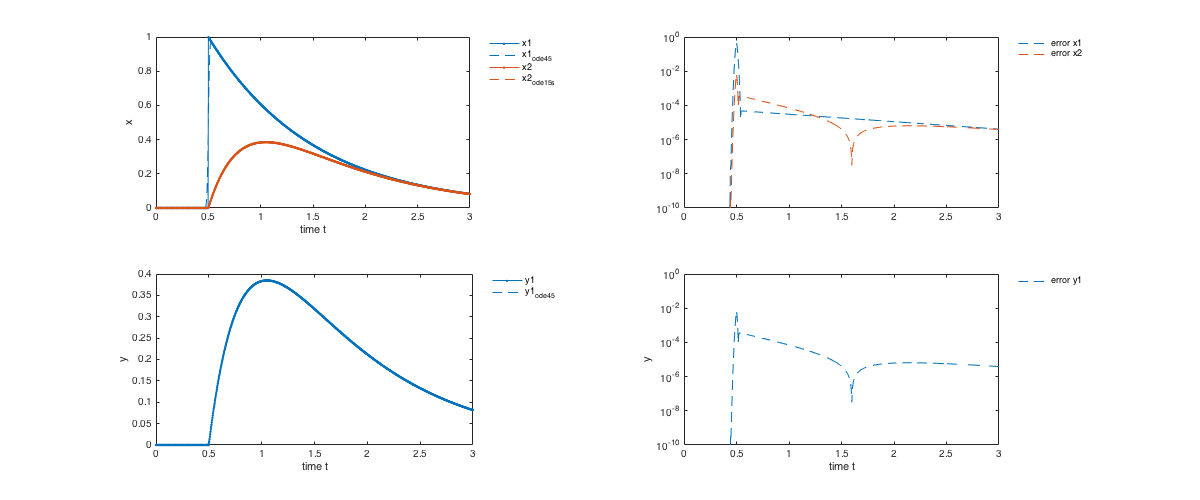
\includegraphics [width=4in]{../../examples/example_2/html/example_model_2_01.png}
\begin{par}
FORWARD SENSITIVITY ANALYSIS
\end{par} \vspace{1em}
\begin{DoxyCode}
options.sensi = 1;

sol = simulate_model_example_2(t,log10(p),k,[],options);
\end{DoxyCode}
\begin{par}
FINITE DIFFERENCES
\end{par} \vspace{1em}
\begin{DoxyCode}
eps = 1e-4;
xi = log10(p);
for ip = 1:4;
    xip = xi;
    xip(ip) = xip(ip) + eps;
    solp = simulate_model_example_2(t,xip,k,[],options);
    sx_fd(:,:,ip) = (solp.x - sol.x)/eps;
    sy_fd(:,:,ip) = (solp.y - sol.y)/eps;
end
\end{DoxyCode}
\begin{par}
PLOTTING
\end{par} \vspace{1em}
\begin{DoxyCode}
figure
for ip = 1:4
    subplot(4,2,ip*2-1)
    hold on
    for ix = 1:size(sol.x,2)
        plot(t,sol.sx(:,ix,ip),'.-','Color',c_x(ix,:))
        plot(t,sx_fd(:,ix,ip),'--','Color',c_x(ix,:))
    end
    ylim([-2,2])
    legend('x1','x1_{fd}','x2','x2_{fd}','Location','NorthEastOutside')
    legend boxoff
    title(['state sensitivity for p' num2str(ip)])
    xlabel('time t')
    ylabel('x')
    box on

    subplot(4,2,ip*2)
    plot(t,abs(sol.sx(:,:,ip)-sx_fd(:,:,ip)),'r--')
    legend('error x1','error x2','Location','NorthEastOutside')
    legend boxoff
    title(['state sensitivity for p' num2str(ip)])
    xlabel('time t')
    ylabel('error')
    ylim([1e-12,1e0])
    set(gca,'YScale','log')
    box on
end
set(gcf,'Position',[100 300 1200 500])

figure
for ip = 1:4
    subplot(4,2,ip*2-1)
    hold on
    for iy = 1:size(sol.y,2)
        plot(t,sol.sy(:,iy,ip),'.-','Color',c_x(iy,:))
        plot(t,sy_fd(:,iy,ip),'--','Color',c_x(iy,:))
    end
    ylim([-2,2])
    legend('y1','y1_{fd}','Location','NorthEastOutside')
    legend boxoff
    title(['observable sensitivity for p' num2str(ip)])
    xlabel('time t')
    ylabel('y')
    box on

    subplot(4,2,ip*2)
    plot(t,abs(sol.sy(:,:,ip)-sy_fd(:,:,ip)),'r--')
    legend('error y1','Location','NorthEastOutside')
    legend boxoff
    title(['observable sensitivity for p' num2str(ip)])
    xlabel('time t')
    ylabel('error')
    ylim([1e-12,1e0])
    set(gca,'YScale','log')
    box on
end
set(gcf,'Position',[100 300 1200 500])
\end{DoxyCode}

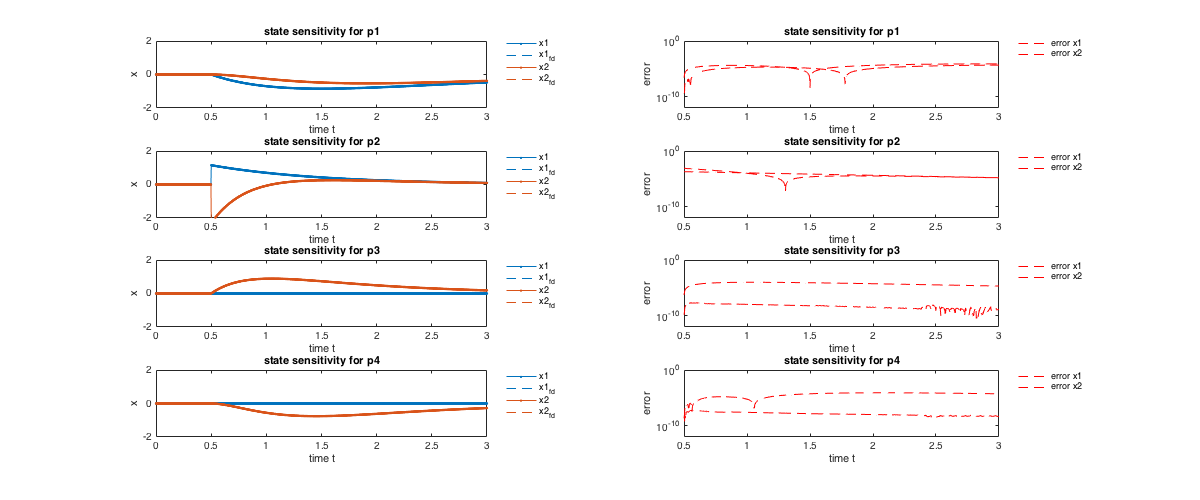
\includegraphics [width=4in]{../../examples/example_2/html/example_model_2_02.png}

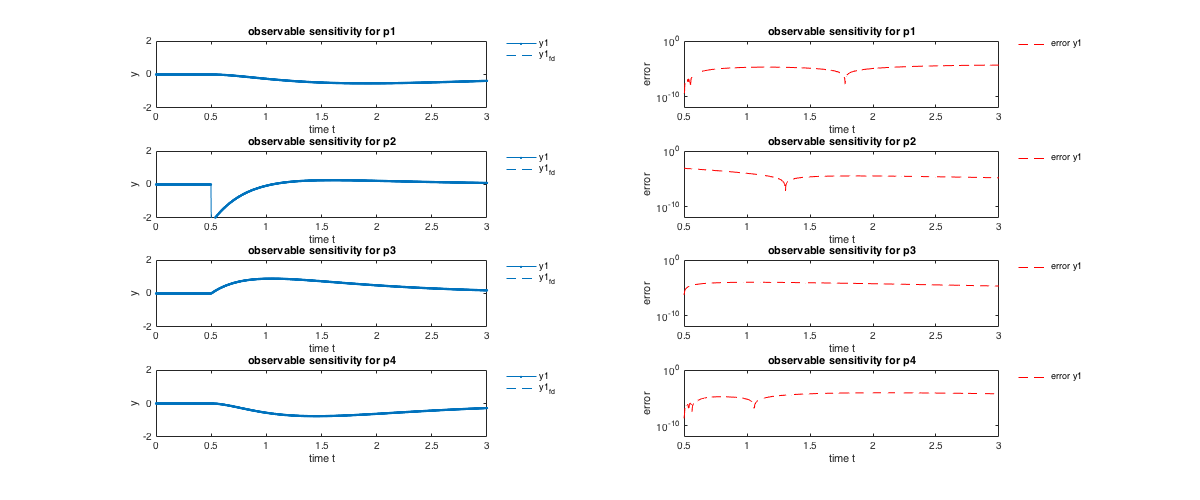
\includegraphics [width=4in]{../../examples/example_2/html/example_model_2_03.png}




     \hypertarget{example3}{}\subsection{Example 3}\label{example3}
\hypertarget{example3_def3}{}\subsubsection{Model Definition}\label{example3_def3}
 
% This LaTeX was auto-generated from MATLAB code.
% To make changes, update the MATLAB code and republish this document.











    
    \begin{DoxyCode}
function [model] = example_model_3_syms()
\end{DoxyCode}
\begin{par}
CVODES OPTIONS
\end{par} \vspace{1em}
\begin{DoxyCode}
% set the default absolute tolerance
model.atol = 1e-8;
% set the default relative tolerance
model.rtol = 1e-8;
% set the default maximum number of integration steps
model.maxsteps = 1e4;
% set the parametrisation of the problem options are 'log', 'log10' and
% 'lin' (default).
model.param = 'log10';
\end{DoxyCode}
\begin{par}
STATES
\end{par} \vspace{1em}
\begin{DoxyCode}
% create state syms
syms x1 x2 x3

% create state vector
x = [
x1 x2 x3
];
\end{DoxyCode}
\begin{par}
PARAMETERS ( for these sensitivities will be computed )
\end{par} \vspace{1em}
\begin{DoxyCode}
% create parameter syms
syms p1 p2 p3 p4 p5

% create parameter vector
p = [p1,p2,p3,p4,p5];
\end{DoxyCode}
\begin{par}
CONSTANTS ( for these no sensitivities will be computed ) this part is optional and can be ommited
\end{par} \vspace{1em}
\begin{DoxyCode}
% create parameter syms
syms k1 k2 k3 k4

% create parameter vector
k = [k1 k2 k3 k4];
\end{DoxyCode}
\begin{par}
SYSTEM EQUATIONS
\end{par} \vspace{1em}
\begin{DoxyCode}
% create symbolic variable for time
syms t

xdot = sym(zeros(size(x)));

% piecewise defined function
xdot(1) = -2*p1*x1^2 - p2*x1*x2 + 2*p3*x2 + p4*x3 + p5;
% inhomogeneous
xdot(2) = +p1*x1^2 - p2*x1*x2 - p3*x2 + p4*x3;
xdot(3) = p2*x1*x2 - p4*x(3) - k4*x(3);
\end{DoxyCode}
\begin{par}
INITIAL CONDITIONS
\end{par} \vspace{1em}
\begin{DoxyCode}
x0 = sym(zeros(size(x)));

x0(1) = k1;
x0(2) = k2;
x0(3) = k3;
\end{DoxyCode}
\begin{par}
OBSERVALES
\end{par} \vspace{1em}
\begin{DoxyCode}
y = sym(zeros(1,1));

y = x;
\end{DoxyCode}
\begin{par}
SYSTEM STRUCT
\end{par} \vspace{1em}
\begin{DoxyCode}
model.sym.x = x;
model.sym.k = k;
model.sym.xdot = xdot;
model.sym.p = p;
model.sym.x0 = x0;
model.sym.y = y;
\end{DoxyCode}
\begin{DoxyCode}
end
\end{DoxyCode}

         \begin{DoxyCode}ans = 
        atol: 1e-08
        rtol: 1e-08
    maxsteps: 10000
       param: 'log10'
         sym: [1x1 struct]
\end{DoxyCode} 
    



    \hypertarget{example3_simu3}{}\subsubsection{Simulation}\label{example3_simu3}
 
% This LaTeX was auto-generated from MATLAB code.
% To make changes, update the MATLAB code and republish this document.











    
    \begin{DoxyCode}
clear
\end{DoxyCode}
\begin{par}
COMPILATION
\end{par} \vspace{1em}
\begin{DoxyCode}
[exdir,~,~]=fileparts(which('example_model_3.m'));
% compile the model
amiwrap('model_example_3','example_model_3_syms',exdir)
% add the model to the path
addpath(genpath([strrep(which('amiwrap.m'),'amiwrap.m','') 'models/model_example_3']))
\end{DoxyCode}

         \begin{DoxyCode}Generating model struct ...
Parsing model struct ...
Generating C code ...
headers | wrapfunctions | 
Compiling mex file ...
Building with 'Xcode with Clang'.
MEX completed successfully.
\end{DoxyCode} 
    \begin{par}
SIMULATION
\end{par} \vspace{1em}
\begin{DoxyCode}
% time vector
t = linspace(0,300,20);
p = [1;0.5;0.4;2;0.1];
k = [0.1,0.4,0.7,1];

options.sensi = 0;
options.cvode_maxsteps = 1e6;
% load mex into memory
sol = simulate_model_example_3(t,log10(p),k,[],options);

tic
sol = simulate_model_example_3(t,log10(p),k,[],options);
disp(['Time elapsed with cvodes: ' num2str(toc) ])
\end{DoxyCode}

         \begin{DoxyCode}Time elapsed with cvodes: 0.002146
\end{DoxyCode} 
    \begin{par}
ODE15S
\end{par} \vspace{1em}
\begin{DoxyCode}
ode_system = @(t,x,p,k) [-2*p(1)*x(1)^2 - p(2)*x(1)*x(2) + 2*p(3)*x(2) + p(4)*x(3) + p(5);
    + p(1)*x(1)^2 - p(2)*x(1)*x(2) - p(3)*x(2) + p(4)*x(3);
    + p(2)*x(1)*x(2) - p(4)*x(3) - k(4)*x(3)];
options_ode15s = odeset('RelTol',1e-8,'AbsTol',1e-8,'MaxStep',1e4);

tic
[~, X_ode15s] = ode15s(@(t,x) ode_system(t,x,p,k),t,k(1:3),options_ode15s);
disp(['Time elapsed with ode15s: ' num2str(toc) ])
\end{DoxyCode}

         \begin{DoxyCode}Time elapsed with ode15s: 0.18018
\end{DoxyCode} 
    \begin{par}
PLOTTING
\end{par} \vspace{1em}
\begin{DoxyCode}
figure
c_x = get(gca,'ColorOrder');
subplot(2,2,1)
for ix = 1:size(sol.x,2)
    plot(t,sol.x(:,ix),'.-','Color',c_x(ix,:))
    hold on
    plot(t,X_ode15s(:,ix),'d','Color',c_x(ix,:))
end
legend('x1','x1_{ode15s}','x2','x2_{ode15s}','x3','x3_{ode15s}','Location','NorthEastOutside')
legend boxoff
xlabel('time t')
ylabel('x')
box on
subplot(2,2,2)
plot(t,abs(sol.x-X_ode15s),'--')
set(gca,'YScale','log')
legend('error x1','error x2','error x3','Location','NorthEastOutside')
legend boxoff
set(gcf,'Position',[100 300 1200 500])
\end{DoxyCode}

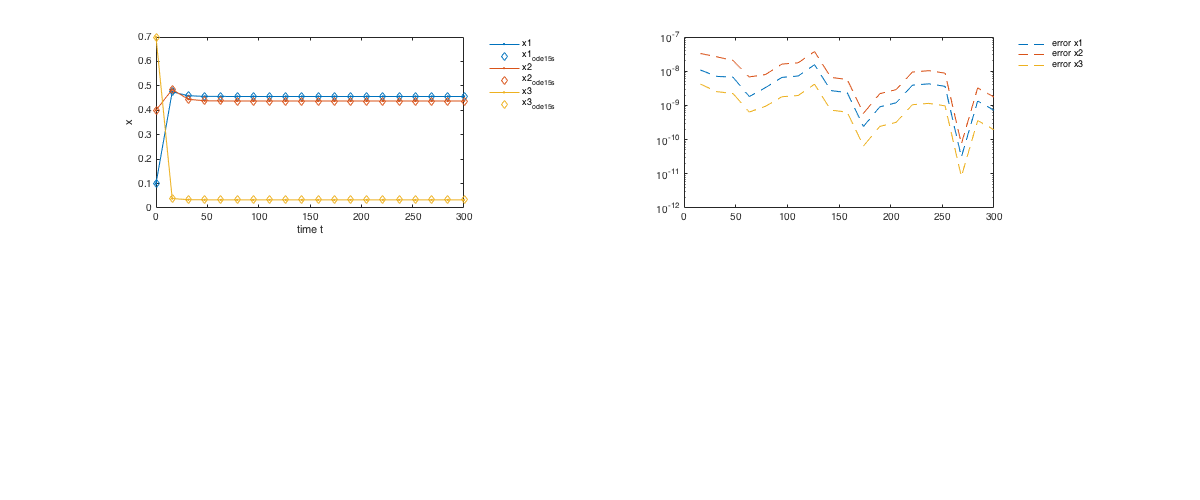
\includegraphics [width=4in]{../../examples/example_3/html/example_model_3_01.png}
\begin{par}
FORWARD SENSITIVITY ANALYSIS
\end{par} \vspace{1em}
\begin{DoxyCode}
options.sensi = 1;
options.sens_ind = [3,1,2,4];

sol = simulate_model_example_3(t,log10(p),k,[],options);
\end{DoxyCode}
\begin{par}
FINITE DIFFERENCES
\end{par} \vspace{1em}
\begin{DoxyCode}
eps = 1e-3;

xi = log10(p);
for ip = 1:4;
    xip = xi;
    xip(ip) = xip(ip) + eps;
    solp = simulate_model_example_3(t,xip,k,[],options);
    sx_fd(:,:,ip) = (solp.x - sol.x)/eps;
    sy_fd(:,:,ip) = (solp.y - sol.y)/eps;
end
\end{DoxyCode}
\begin{par}
PLOTTING
\end{par} \vspace{1em}
\begin{DoxyCode}
figure
for ip = 1:4
    subplot(4,2,ip*2-1)
    hold on
    for ix = 1:size(sol.x,2)
        plot(t,sol.sx(:,ix,ip),'.-','Color',c_x(ix,:))
        plot(t,sx_fd(:,ix,options.sens_ind(ip)),'d','Color',c_x(ix,:))
    end
    legend('x1','x1_{fd}','x2','x2_{fd}','x3','x3_{fd}','Location','NorthEastOutside')
    legend boxoff
    title(['state sensitivity for p' num2str(options.sens_ind(ip))])
    xlabel('time t')
    ylabel('x')
    box on

    subplot(4,2,ip*2)
    plot(t,abs(sol.sx(:,:,ip)-sx_fd(:,:,options.sens_ind(ip))),'--')
    legend('error x1','error x2','error x3','Location','NorthEastOutside')
    legend boxoff
    title(['error of state sensitivity for p' num2str(options.sens_ind(ip))])
    xlabel('time t')
    ylabel('error')
    set(gca,'YScale','log')
    box on
end
set(gcf,'Position',[100 300 1200 500])
\end{DoxyCode}

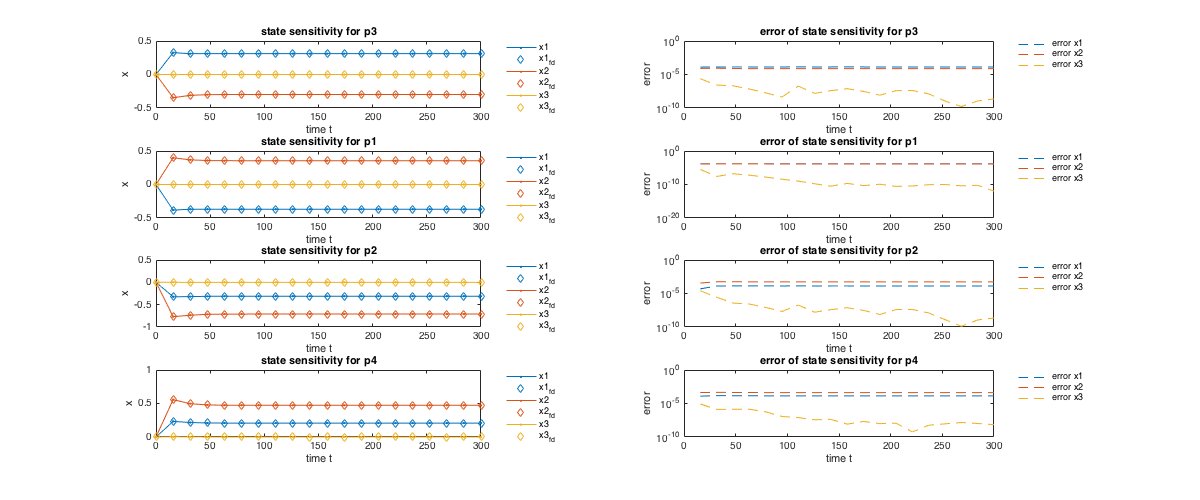
\includegraphics [width=4in]{../../examples/example_3/html/example_model_3_02.png}
\begin{par}
STEADY STATE SENSITIVITY
\end{par} \vspace{1em}
\begin{DoxyCode}
sssens = NaN(size(sol.sx));
for it = 2:length(t)
    tt = [0,t(it)];
    options.sensi_meth = 'ss';
    solss = simulate_model_example_3(tt,log10(p),k,[],options);
    sssens(it,:,:) = solss.sx;
    ssxdot(it,:) = solss.xdot;
end
\end{DoxyCode}
\begin{par}
PLOTTING
\end{par} \vspace{1em}
\begin{DoxyCode}
figure
for ip = 1:4
    subplot(4,2,ip*2-1)
    hold on
    for ix = 1:size(sol.x,2)
        plot(t,sol.sx(:,ix,ip),'.-','Color',c_x(ix,:))
        plot(t,sssens(:,ix,ip),'d-','Color',c_x(ix,:))
    end
    legend('x1','x1_{ss}','x2','x2_{ss}','x3','x3_{ss}','Location','NorthEastOutside')
    legend boxoff
    title(['state steady sensitivity for p' num2str(ip)])
    xlabel('time t')
    ylabel('x')
    box on

    subplot(4,2,ip*2)
    plot(t,abs(sol.sx(:,:,ip)-sssens(:,:,ip)),'--')
    legend('error x1','error x2','error x3','Location','NorthEastOutside')
    legend boxoff
    title(['error of steady state sensitivity for p' num2str(ip)])
    xlabel('time t')
    ylabel('error')
    set(gca,'YScale','log')
    box on
end
set(gcf,'Position',[100 300 1200 500])

figure
scatter(sqrt(sum((ssxdot./sol.x).^2,2)),sqrt(sum(sum((sol.sx-sssens).^2,2),3)))
hold on
plot([1e-15,1e5],[1e-15,1e5],'k:')
set(gca,'YScale','log')
set(gca,'XScale','log')
box on
axis square
xlabel('||dxdt/x||_2')
ylabel('error steady state approximation')
set(gca,'FontSize',15)
set(gca,'LineWidth',1.5)
set(gcf,'Position',[100 300 1200 500])
\end{DoxyCode}

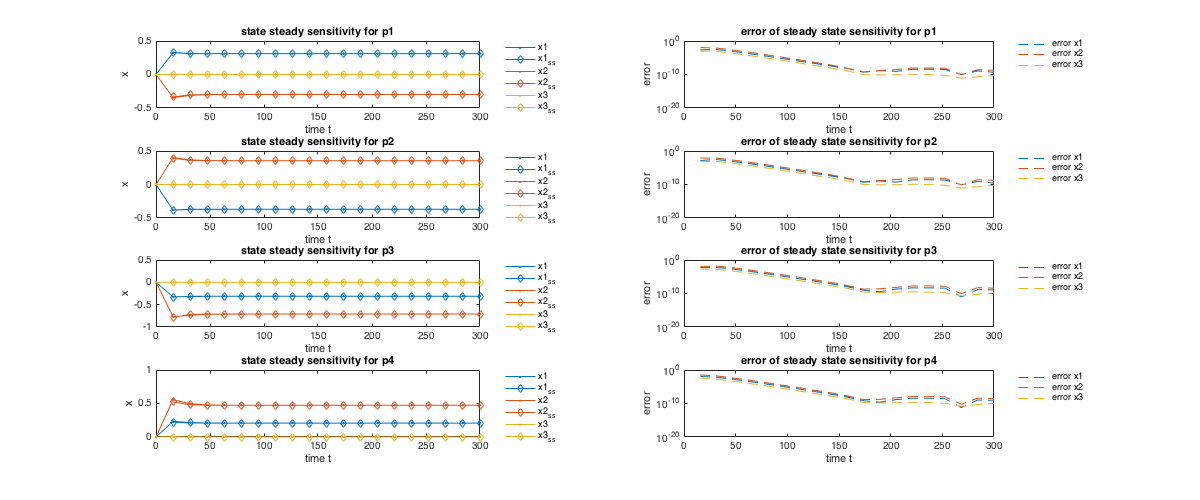
\includegraphics [width=4in]{../../examples/example_3/html/example_model_3_03.png}

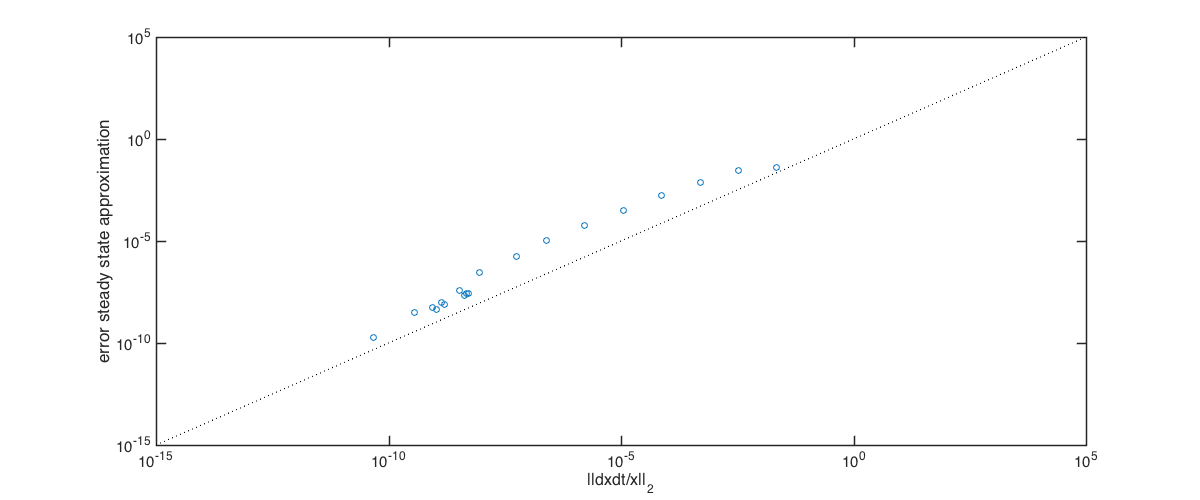
\includegraphics [width=4in]{../../examples/example_3/html/example_model_3_04.png}




     \hypertarget{example4}{}\subsection{Example 4}\label{example4}
\hypertarget{example4_def4}{}\subsubsection{Model Definition}\label{example4_def4}
 
% This LaTeX was auto-generated from MATLAB code.
% To make changes, update the MATLAB code and republish this document.











    
    \begin{DoxyCode}
function [model] = example_model_4_syms()
\end{DoxyCode}
\begin{par}
CVODES OPTIONS
\end{par} \vspace{1em}
\begin{DoxyCode}
model.atol = 1e-12;
model.rtol = 1e-8;
model.maxsteps = 1e4;
model.param = 'log10';
\end{DoxyCode}
\begin{par}
STATES
\end{par} \vspace{1em}
\begin{DoxyCode}
syms STAT pSTAT pSTAT_pSTAT npSTAT_npSTAT nSTAT1 nSTAT2 nSTAT3 nSTAT4 nSTAT5

x = [
STAT, pSTAT, pSTAT_pSTAT, npSTAT_npSTAT, nSTAT1, nSTAT2, nSTAT3, nSTAT4, nSTAT5 ...
];
\end{DoxyCode}
\begin{par}
PARAMETERS
\end{par} \vspace{1em}
\begin{DoxyCode}
syms p1 p2 p3 p4 init_STAT Omega_cyt Omega_nuc sp1 sp2 sp3 sp4 sp5 offset_tSTAT offset_pSTAT scale_tSTAT scale_pSTAT sigma_pSTAT sigma_tSTAT sigma_pEpoR

p = [p1,p2,p3,p4,init_STAT,sp1,sp2,sp3,sp4,sp5,offset_tSTAT,offset_pSTAT,scale_tSTAT,scale_pSTAT,sigma_pSTAT,sigma_tSTAT,sigma_pEpoR];

k = [Omega_cyt,Omega_nuc];
\end{DoxyCode}
\begin{par}
INPUT
\end{par} \vspace{1em}
\begin{DoxyCode}
syms t
u(1) = spline_pos5(t, 0.0, sp1, 5.0, sp2, 10.0, sp3, 20.0, sp4, 60.0, sp5, 0, 0.0);
\end{DoxyCode}
\begin{par}
SYSTEM EQUATIONS
\end{par} \vspace{1em}
\begin{DoxyCode}
xdot = sym(zeros(size(x)));

xdot(1) = (Omega_nuc*p4*nSTAT5 - Omega_cyt*STAT*p1*u(1))/Omega_cyt;
xdot(2) = STAT*p1*u(1) - 2*p2*pSTAT^2;
xdot(3) = p2*pSTAT^2 - p3*pSTAT_pSTAT;
xdot(4) = -(Omega_nuc*p4*npSTAT_npSTAT - Omega_cyt*p3*pSTAT_pSTAT)/Omega_nuc;
xdot(5) = -p4*(nSTAT1 - 2*npSTAT_npSTAT);
xdot(6) = p4*(nSTAT1 - nSTAT2);
xdot(7) = p4*(nSTAT2 - nSTAT3);
xdot(8) = p4*(nSTAT3 - nSTAT4);
xdot(9) = p4*(nSTAT4 - nSTAT5);
\end{DoxyCode}
\begin{par}
INITIAL CONDITIONS
\end{par} \vspace{1em}
\begin{DoxyCode}
x0 = sym(zeros(size(x)));

x0(1) = init_STAT;
\end{DoxyCode}
\begin{par}
OBSERVABLES
\end{par} \vspace{1em}
\begin{DoxyCode}
y = sym(zeros(3,1));

y(1) = offset_pSTAT + scale_pSTAT/init_STAT*(pSTAT + 2*pSTAT_pSTAT);
y(2) = offset_tSTAT + scale_tSTAT/init_STAT*(STAT + pSTAT + 2*(pSTAT_pSTAT));
y(3) = u(1);
\end{DoxyCode}
\begin{par}
SIGMA
\end{par} \vspace{1em}
\begin{DoxyCode}
sigma_y = sym(size(y));

sigma_y(1) = sigma_pSTAT;
sigma_y(2) = sigma_tSTAT;
sigma_y(3) = sigma_pEpoR;
\end{DoxyCode}
\begin{par}
SYSTEM STRUCT
\end{par} \vspace{1em}
\begin{DoxyCode}
model.sym.x = x;
model.sym.u = u;
model.sym.xdot = xdot;
model.sym.p = p;
model.sym.k = k;
model.sym.x0 = x0;
model.sym.y = y;
model.sym.sigma_y = sigma_y;
\end{DoxyCode}
\begin{DoxyCode}
end
\end{DoxyCode}

         \begin{DoxyCode}ans = 
        atol: 1e-12
        rtol: 1e-08
    maxsteps: 10000
       param: 'log10'
         sym: [1x1 struct]
\end{DoxyCode} 
    



    \hypertarget{example4_simu4}{}\subsubsection{Simulation}\label{example4_simu4}
 
% This LaTeX was auto-generated from MATLAB code.
% To make changes, update the MATLAB code and republish this document.











    
    \begin{DoxyCode}
clear
% compile the model
[exdir,~,~]=fileparts(which('example_model_4.m'));
amiwrap('model_example_4','example_model_4_syms',exdir)

num = xlsread(fullfile(exdir,'pnas_data_original.xls'));

t = num(:,1);

D.Y = num(:,[2,4,6]);
D.Sigma_Y = NaN(size(D.Y));


kappa = [1.4,0.45];

xi =  [0.595102743982229
    2.99999999999997
    -0.948930681736172
    -0.00751433662124028
    0
    -2.78593598707493
    -0.256066441623149
    -0.07511250551843
    -0.411247187909784
    -4.99999999959546
    -0.735327875726678
    -0.64146041506584
    -0.107897525629158
    0.0272647740863191
    -0.5
    0
    -0.5];

options.sensi = 0;
sol = simulate_model_example_4(t,xi,kappa,D,options);

figure
for iy = 1:3
    subplot(2,2,iy)
    plot(t,D.Y(:,iy),'rx')
    hold on
    plot(t,sol.y(:,iy),'.-')
    xlim([0,60])
    xlabel('t')
    switch(iy)
        case 1
            ylabel('pStat')
        case 2
            ylabel('tStat')
        case 3
            ylabel('pEpoR')
    end
    ylim([0,1.2])
end
set(gcf,'Position',[100 300 1200 500])

% generate new
xi_rand = xi + 0.1;
options.sensi = 1;
options.sensi_meth = 'adjoint';
sol = simulate_model_example_4(t,xi_rand,kappa,D,options);

options.sensi = 0;
eps = 1e-4;
fd_grad = NaN(length(xi),1);
for ip = 1:length(xi)
    xip = xi_rand;
    xip(ip) = xip(ip) + eps;
    psol = simulate_model_example_4(t,xip,kappa,D,options);
    fd_grad(ip) = (psol.llh-sol.llh)/eps;
end

figure
scatter(abs(sol.sllh),abs(fd_grad))
set(gca,'XScale','log')
set(gca,'YScale','log')
xlim([1e-2,1e2])
ylim([1e-2,1e2])
box on
hold on
axis square
plot([1e-2,1e2],[1e-2,1e2],'k:')
xlabel('adjoint sensitivity absolute value of gradient element')
ylabel('finite difference absolute value of gradient element')
set(gcf,'Position',[100 300 1200 500])
\end{DoxyCode}

         \begin{DoxyCode}Generating model struct ...
Parsing model struct ...
Generating C code ...
headers | wrapfunctions | 
Compiling mex file ...
Building with 'Xcode with Clang'.
MEX completed successfully.
\end{DoxyCode} 
    
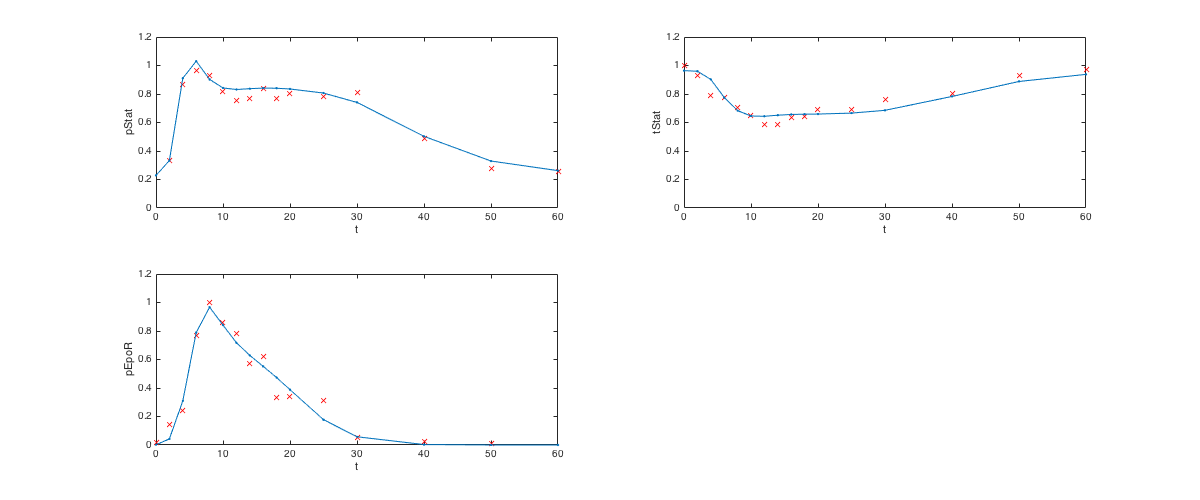
\includegraphics [width=4in]{../../examples/example_4/html/example_model_4_01.png}

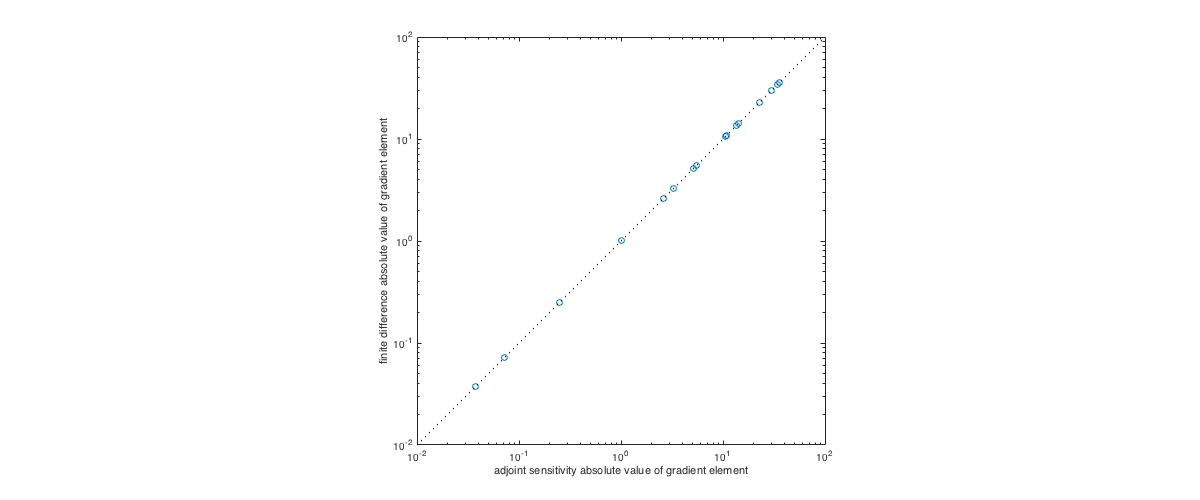
\includegraphics [width=4in]{../../examples/example_4/html/example_model_4_02.png}




     \hypertarget{example5}{}\subsection{Example 5}\label{example5}
\hypertarget{example5_def5}{}\subsubsection{Model Definition}\label{example5_def5}
 
% This LaTeX was auto-generated from MATLAB code.
% To make changes, update the MATLAB code and republish this document.











    
    \begin{DoxyCode}
function [model] = example_model_5_syms()
\end{DoxyCode}
\begin{par}
CVODES OPTIONS
\end{par} \vspace{1em}
\begin{DoxyCode}
% set the default absolute tolerance
model.atol = 1e-8;
% set the default relative tolerance
model.rtol = 1e-8;
% set the default maximum number of integration steps
model.maxsteps = 1e4;
% set the parametrisation of the problem options are 'log', 'log10' and
% 'lin' (default).
model.param = 'log10';
\end{DoxyCode}
\begin{par}
STATES
\end{par} \vspace{1em}
\begin{DoxyCode}
% create state syms
syms x1 x2

% create state vector
x = [ x1 x2 ];
\end{DoxyCode}
\begin{par}
PARAMETERS ( for these sensitivities will be computed )
\end{par} \vspace{1em}
\begin{DoxyCode}
% create parameter syms
syms p1 p2 p3 p4

% create parameter vector
p = [p1,p2,p3,p4];
\end{DoxyCode}
\begin{par}
SYSTEM EQUATIONS
\end{par} \vspace{1em}
\begin{DoxyCode}
% create symbolic variable for time
syms t

xdot = sym(zeros(size(x)));

% piecewise defined function
xdot(1) = -p1*x1 + dirac(t-p2);
% inhomogeneous
xdot(2) = p3*x1 - p4*x2 ;
\end{DoxyCode}
\begin{par}
INITIAL CONDITIONS
\end{par} \vspace{1em}
\begin{DoxyCode}
x0 = sym(zeros(size(x)));

x0(1) = 0;
x0(2) = 0;
\end{DoxyCode}
\begin{par}
OBSERVALES
\end{par} \vspace{1em}
\begin{DoxyCode}
y = sym(zeros(1,1));

y(1) = x2;
\end{DoxyCode}
\begin{par}
SYSTEM STRUCT
\end{par} \vspace{1em}
\begin{DoxyCode}
model.sym.x = x;
model.sym.xdot = xdot;
model.sym.p = p;
model.sym.x0 = x0;
model.sym.y = y;
\end{DoxyCode}
\begin{DoxyCode}
end
\end{DoxyCode}

         \begin{DoxyCode}ans = 
        atol: 1e-08
        rtol: 1e-08
    maxsteps: 10000
       param: 'log10'
         sym: [1x1 struct]
\end{DoxyCode} 
    



    \hypertarget{example5_simu5}{}\subsubsection{Simulation}\label{example5_simu5}
 
% This LaTeX was auto-generated from MATLAB code.
% To make changes, update the MATLAB code and republish this document.











    
    \begin{DoxyCode}
clear
\end{DoxyCode}
\begin{par}
COMPILATION
\end{par} \vspace{1em}
\begin{DoxyCode}
[exdir,~,~]=fileparts(which('example_model_5.m'));
% compile the model
amiwrap('model_example_5','example_model_5_syms',exdir)
\end{DoxyCode}

         \begin{DoxyCode}Generating model struct ...
Parsing model struct ...
Generating C code ...
headers | wrapfunctions | 
Compiling mex file ...
Building with 'Xcode with Clang'.
MEX completed successfully.
\end{DoxyCode} 
    \begin{par}
SIMULATION
\end{par} \vspace{1em}
\begin{DoxyCode}
% time vector
tout = linspace(0,4,9);
tfine = linspace(0,4,10001);
p = [1;0.4;2;3];
k = [];

D.Y = [  0.00714742903826096
      -0.00204966058299775
         0.382159034587845
          0.33298932672138
         0.226111476113441
         0.147028440865854
        0.0882468698791813
        0.0375887796628869
        0.0373422340295005];

D.Sigma_Y = 0.01*ones(size(D.Y));


options.sensi = 1;
options.sensi_meth = 'adjoint';
options.cvode_maxsteps = 1e4;
sol = simulate_model_example_5(tout,log10(p),k,D,options);
options.sensi = 0;
solfine = simulate_model_example_5(tfine,log10(p),k,[],options);

figure
errorbar(tout,D.Y,D.Sigma_Y)
hold on
plot(tfine,solfine.y)
legend('data','simulation')
xlabel('time t')
ylabel('observable')
title(['log-likelihood: ' num2str(sol.llh) ])
\end{DoxyCode}

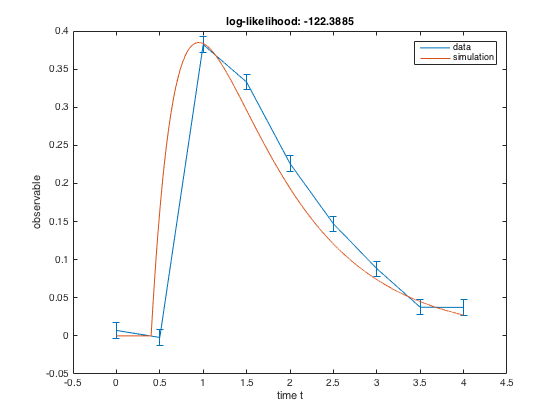
\includegraphics [width=4in]{../../examples/example_5/html/example_model_5_01.png}
\begin{par}
FD
\end{par} \vspace{1em}
\begin{DoxyCode}
eps = 1e-4;
xi = log10(p);
grad_fd_f = NaN(4,1);
grad_fd_b = NaN(4,1);
for ip = 1:4;
    options.sensi = 0;
    xip = xi;
    xip(ip) = xip(ip) + eps;
    solpf = simulate_model_example_5(tout,xip,k,D,options);
    grad_fd_f(ip,1) = (solpf.llh-sol.llh)/eps;
    xip = xi;
    xip(ip) = xip(ip) - eps;
    solpb = simulate_model_example_5(tout,xip,k,D,options);
    grad_fd_b(ip,1) = -(solpb.llh-sol.llh)/eps;
end

figure
plot(abs(grad_fd_f),abs(sol.sllh),'o')
hold on
plot(abs(grad_fd_b),abs(sol.sllh),'o')
set(gca,'XScale','log')
set(gca,'YScale','log')
hold on
axis square
plot([1e2,1e4],[1e2,1e4],'k:')
xlim([1e2,1e4])
ylim([1e2,1e4])
legend('forward FD','backward FD','Location','SouthEast')
xlabel('adjoint sensitivity absolute value of gradient element')
ylabel('computed absolute value of gradient element')
set(gcf,'Position',[100 300 1200 500])
\end{DoxyCode}

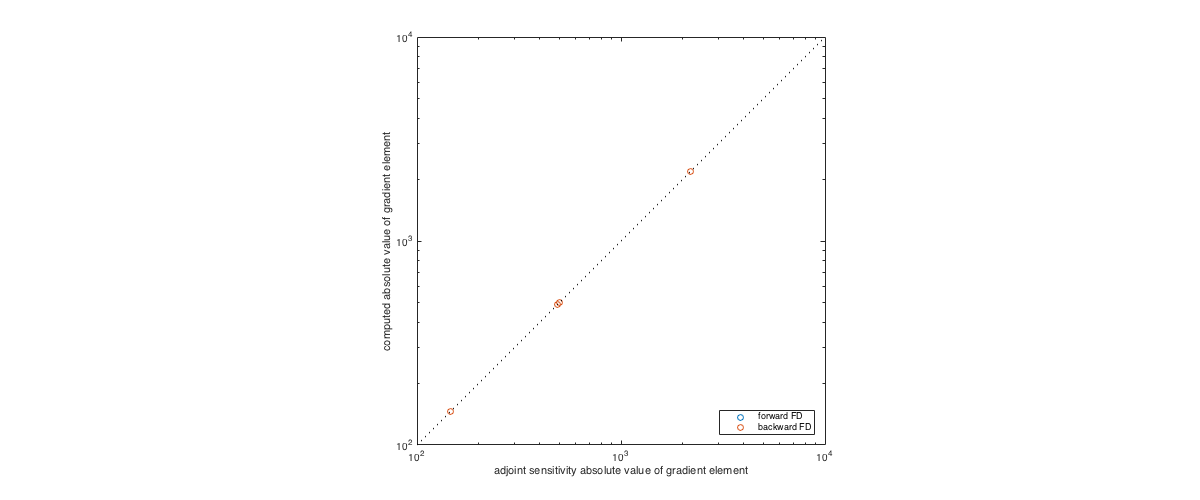
\includegraphics [width=4in]{../../examples/example_5/html/example_model_5_02.png}




     \hypertarget{example6}{}\subsection{Example 6}\label{example6}
\hypertarget{example6_def6}{}\subsubsection{Model Definition}\label{example6_def6}
 
% This LaTeX was auto-generated from MATLAB code.
% To make changes, update the MATLAB code and republish this document.











    
    \begin{DoxyCode}
function [model] = example_model_6_syms()
\end{DoxyCode}
\begin{par}
CVODES OPTIONS
\end{par} \vspace{1em}
\begin{DoxyCode}
% set the default absolute tolerance
model.atol = 1e-8;
% set the default relative tolerance
model.rtol = 1e-8;
% set the default maximum number of integration steps
model.maxsteps = 1e4;
% set the parametrisation of the problem options are 'log', 'log10' and
% 'lin' (default).
model.param = 'log10';
\end{DoxyCode}
\begin{par}
STATES
\end{par} \vspace{1em}
\begin{DoxyCode}
% create state syms
syms x1

% create state vector
x = [ x1];
\end{DoxyCode}
\begin{par}
PARAMETERS ( for these sensitivities will be computed )
\end{par} \vspace{1em}
\begin{DoxyCode}
% create parameter syms
syms p1 p2 p3

% create parameter vector
p = [p1 p2 p3];
\end{DoxyCode}
\begin{par}
SYSTEM EQUATIONS
\end{par} \vspace{1em}
\begin{DoxyCode}
% create symbolic variable for time
syms t

xdot = sym(zeros(size(x)));

% piecewise defined function
xdot(1) = -p1*x1*heaviside(t-2) + p2;
\end{DoxyCode}
\begin{par}
INITIAL CONDITIONS
\end{par} \vspace{1em}
\begin{DoxyCode}
x0 = sym(zeros(size(x)));

x0(1) = p3;
\end{DoxyCode}
\begin{par}
OBSERVALES
\end{par} \vspace{1em}
\begin{DoxyCode}
y = sym(zeros(1,1));

y(1) = x1;
\end{DoxyCode}
\begin{par}
SYSTEM STRUCT
\end{par} \vspace{1em}
\begin{DoxyCode}
model.sym.x = x;
model.sym.xdot = xdot;
model.sym.p = p;
model.sym.x0 = x0;
model.sym.y = y;
\end{DoxyCode}
\begin{DoxyCode}
end
\end{DoxyCode}

         \begin{DoxyCode}ans = 
        atol: 1e-08
        rtol: 1e-08
    maxsteps: 10000
       param: 'log10'
         sym: [1x1 struct]
\end{DoxyCode} 
    



    \hypertarget{example6_simu6}{}\subsubsection{Simulation}\label{example6_simu6}
 
% This LaTeX was auto-generated from MATLAB code.
% To make changes, update the MATLAB code and republish this document.











    
    \begin{DoxyCode}
clear
\end{DoxyCode}
\begin{par}
COMPILATION
\end{par} \vspace{1em}
\begin{DoxyCode}
[exdir,~,~]=fileparts(which('example_model_6.m'));
% compile the model
amiwrap('model_example_6','example_model_6_syms',exdir)
\end{DoxyCode}

         \begin{DoxyCode}Generating model struct ...
Parsing model struct ...
Generating C code ...
headers | wrapfunctions | 
Compiling mex file ...
Building with 'Xcode with Clang'.
MEX completed successfully.
\end{DoxyCode} 
    \begin{par}
SIMULATION
\end{par} \vspace{1em}
\begin{DoxyCode}
% time vector
t = [linspace(0,4,5)];
p = [1.1,0.3,1];
k = [];

% D.Y = [     1.0171
%     1.1761
%     1.1680
%     1.1359
%     1.1778
%     1.3423
%     1.3079
%     1.2784
%     1.4976
%     1.5903
%     1.6585
%     1.4688
%     1.0999
%     1.0128
%     0.7198
%     0.9814
%     0.6755
%     0.5091
%     0.4471
%     0.5249
%     0.3288];


D.Y = [     1.0171
    1.3423
    1.6585
    0.9814
    0.3288];

D.Sigma_Y = 0.1*ones(size(D.Y));


options.sensi = 1;
options.sensi_meth = 'adjoint';
options.cvode_maxsteps = 1e6;
options.cvode_rtol = 1e-12;
options.cvode_atol = 1e-12;
% load mex into memory
[msg] = which('simulate_model_example_6'); % fix for inaccessability problems
sol = simulate_model_example_6(t,log10(p),k,D,options);
\end{DoxyCode}
\begin{par}
Plot
\end{par} \vspace{1em}
\begin{DoxyCode}
figure
subplot(3,1,1)
errorbar(t,D.Y,D.Sigma_Y)
hold on
% plot(t,sol.y)

xlabel('time t')
ylabel('observable')
title(['log-likelihood: ' num2str(sol.llh) ])

y = (p(2)*t + p(3)).*(t<2) + ( (2*p(2)+p(3)-p(2)/p(1))*exp(-p(1)*(t-2))+p(2)/p(1) ).*(t>=2);


tfine = linspace(0,4,100001);
xfine = (p(2)*tfine + 1).*(tfine<2) + ( (2*p(2)+p(3)-p(2)/p(1))*exp(-p(1)*(tfine-2))+p(2)/p(1) ).*(tfine>=2);

mu = zeros(1,length(tfine));
for it = 1:length(t)
if(t(it)<=2)
mu = mu + ((y(it)-D.Y(it))/(D.Sigma_Y(it)^2))*(tfine<=t(it));
else
mu = mu + ((y(it)-D.Y(it))/(D.Sigma_Y(it)^2))*exp(p(1)*(tfine-t(it))).*(tfine<=t(it)).*(tfine>2) + ((y(it)-D.Y(it))/(D.Sigma_Y(it)^2))*exp(p(1)*(2-t(it))).*(tfine<t(it)).*(tfine<=2);
end
end
plot(tfine,xfine)
legend('data','simulation')
xlim([min(t)-0.5,max(t)+0.5])
subplot(3,1,2)
plot(tfine,mu)
ylabel('adjoint')
xlabel('time t')
xlim([min(t)-0.5,max(t)+0.5])

subplot(3,1,3)

plot(fliplr(tfine),-cumsum(fliplr(-mu.*xfine.*(tfine>2)))*p(1)*log(10)*(t(end)/numel(tfine)))
hold on
plot(fliplr(tfine),-cumsum(fliplr(mu))*p(2)*log(10)*(t(end)/numel(tfine)))
plot(tfine,-mu(1)*p(3)*log(10)*(tfine<2))
xlim([min(t)-0.5,max(t)+0.5])
ylabel('integral')
xlabel('time t')

legend('p1','p2','p3')

grad(1,1) = -trapz(tfine,-mu.*xfine.*(tfine>2))*p(1)*log(10);
grad(2,1) = -trapz(tfine,mu)*p(2)*log(10);
grad(3,1) = -mu(1)*p(3)*log(10);

plot(zeros(3,1),grad,'ko')
\end{DoxyCode}

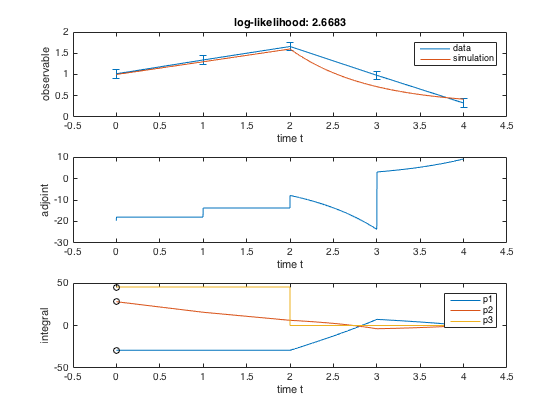
\includegraphics [width=4in]{../../examples/example_6/html/example_model_6_01.png}
\begin{par}
FD
\end{par} \vspace{1em}
\begin{DoxyCode}
eps = 1e-5;
xi = log10(p);
grad_fd_f = NaN(3,1);
grad_fd_b = NaN(3,1);
for ip = 1:3;
    options.sensi = 0;
    xip = xi;
    xip(ip) = xip(ip) + eps;
    solp = simulate_model_example_6(t,xip,k,D,options);
    grad_fd_f(ip,1) = (solp.llh-sol.llh)/eps;
    xip = xi;
    xip(ip) = xip(ip) - eps;
    solp = simulate_model_example_6(t,xip,k,D,options);
    grad_fd_b(ip,1) = -(solp.llh-sol.llh)/eps;
end

figure
plot(abs(grad),abs(grad_fd_f),'o')
hold on
plot(abs(grad),abs(grad_fd_b),'o')
plot(abs(grad),mean([abs(grad_fd_b),abs(grad_fd_f)],2),'o')
plot(abs(grad),abs(sol.sllh),'o')
plot([1e1,1e2],[1e1,1e2],'k:')
set(gca,'XScale','log')
set(gca,'YScale','log')
axis square
legend('forward FD','backward FD','central FD','adjoint sensintivity analysis','Location','SouthEast')
xlabel('analytic absolute value of gradient element')
ylabel('computed absolute value of gradient element')
set(gcf,'Position',[100 300 1200 500])
\end{DoxyCode}

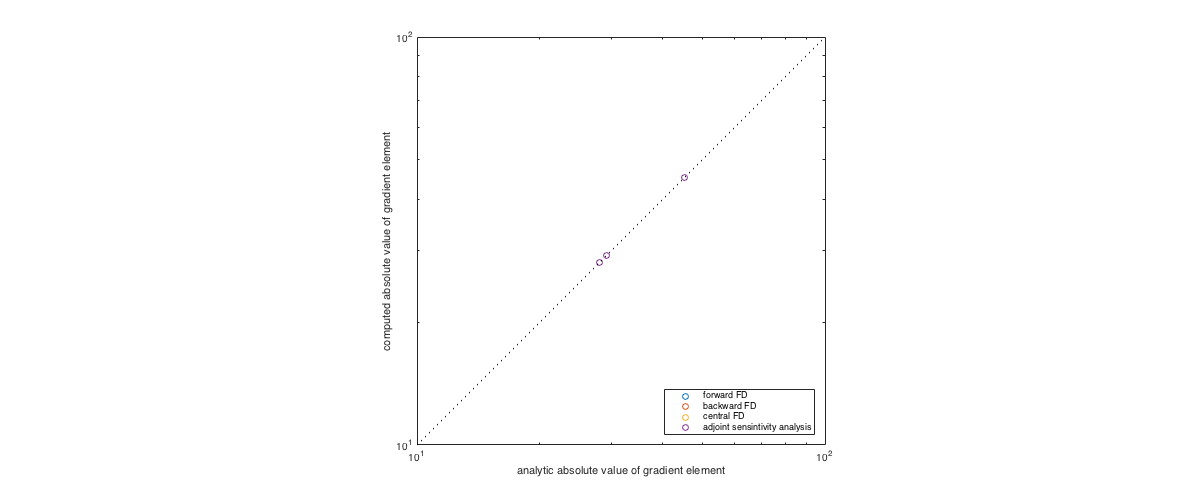
\includegraphics [width=4in]{../../examples/example_6/html/example_model_6_02.png}




     